\documentclass[9pt,a4paper]{article}
\usepackage[latin1]{inputenc}
\usepackage{amsmath}
\usepackage{amsfonts}
\usepackage{amssymb}x
\usepackage{graphicx}
\usepackage{listings}
\usepackage{color}

\definecolor{dkgreen}{rgb}{0,0.6,0}
\definecolor{gray}{rgb}{0.5,0.5,0.5}
\definecolor{mauve}{rgb}{0.58,0,0.82}

\author{Beerend Lauwers and Frank Wijmans}
\title{Project 2: SPIN model checking of a social network}
\begin{document}
	\maketitle
	
	\section{Introduction}
	
	The minimal problem to solve was as follows:
	Build a model for a social network for 4 users with the following social relation:
	\begin{itemize}
		\item User 0 has no followers
		\item User n has two followers, i+x mod 4, for x = 1 and x = 2.
	\end{itemize}
	
	Some restrictions were applied to minimize the state space.
	Furthermore, the requirements for correctness were:
	\begin{enumerate}
		\item Privacy constraints
		\item No deadlocking
		\item Messages will eventually reach its recipients.
	\end{enumerate}
	
	\section{Data definitions}
	In the model we use the following global definitions and data types to build our algorithm upon.
	We define the number of users as 4 and of those four users, one is non-deterministically chosen to send a message.
	
	As for data types, we use channel arrays containing messages of the form of ${byte, byte, byte}$.
	The use of channels was required. 
	We have two channels per user, namely an inbox and an outbox.
	The relation between a user and its channels are identified by the index of the array.
	\begin{center}
		User 1 has $inbox[1]$ and $outbox[1]$ as channels.
	\end{center}
	
	\section{Algorithm}
	
	Our algorithm is based on the following idea:
	\textit{All users have one device, it is a \texttt{proctype} called userDevice which takes a user identification byte as its single parameter.}
	Each user device does three things which are looped in non-deterministic fashion using the \texttt{do} notation.
	\begin{itemize}
		\item \textbf{Creating new messages:} If both the user's inbox and outbox is empty, a message is added to the outbox of the same user.
		\item \textbf{Reading inbox messages:} If the inbox is not empty, a message is removed from the inbox, and if the constraint requires the user to forward the message, then try and forward.
		\begin{enumerate}
			\item \textbf{Forwarding messages:} If it is possible to add another message to the outbox, do so. Otherwise, place the message back in the inbox and try again later. (It will wait for the outbox to be emptied.)
		\end{enumerate}
		\item \textbf{Sending messages:} If the outbox is not empty, take an outbox message, and add the message to the inbox of the direct followers of the user.
	\end{itemize}
	
	\section{Linear time logic formulae}
	We have two LTL formulae to verify the most difficult correctness requirement.
	Namely the requirement that messages eventually reach the followers in the case of an \textit{Fo} message, and reach the followers, and followers of followers if it is a \textit{Fo2} message.
	
	Formulating these requirements in one LTL formula would be an large statement, and would only make it less readable.
	
	We have chosen to define two formulae because we argue that when two runs, one for each of the formulae shows that respective formula is verified, it would imply that both hold as if it were one statement.
	
	First, we defined the formula for \textit{Fo}. The LTL-formula below is to check whether a sent message (at label \texttt{S0}) is eventually read (at label \texttt{R0}) for the first of the two followers by stating $(i+1) \% users$. A similar formula was constructed for the second follower, which uses the label \texttt{S1} and refers to  $(i+2) \% users$. We quantify over the content in the variable k, it is use to check if the content of two messages is the same. Because we are dealing with a historical value when eventually the message is read, we need to use this helper-variable k.
	\begin{align*}
	\forall i, k. 
	\square\ ( & i > 0 \\
	& \wedge\ device[i]@S0 \\
	& \wedge\ device[i]:constraint > 0 ) \\
	& \wedge\ device[i]:content == k ) \\
	\rightarrow & \\
	\Diamond\ ( & device[(i+1) \%  users]@R0 \\
	& \wedge\ device[(i+1) \% users]:content == k)
	\end{align*}
	
	For the constraint of \textit{Fo2} we have a formula that resembles the formula above. It may be clear that we have to not only check the two followers, but also the followers of those two.
	And we have to make sure that the followers are not user 0, as since user 0 does not have followers, they will never forward a message. Again, the formula below is only a part of the entire formula, where we check the two followers of a follower of the sender.
	\begin{align*}
	\forall i, k. 
	\square\ ( & i > 0 \\
	& \wedge\ device[i]@S0 \\
	& \wedge\ device[i]:constraint == 2 \\
	& \wedge\ device[i]:content == k \\
	& \wedge\ ((i+1)\%users) > 0) \\
	\rightarrow\ & \\
	\Diamond\ ( & device[(((i+1) \% users)+1) \%  users]@R0 \\
	& \wedge\ device[(((i+1) \% users)+1) \%  users]:content == k \\
	& device[(((i+1) \% users)+2) \%  users]@R0 \\
	& \wedge\ device[(((i+1) \% users)+2) \%  users]:content == k)
	\end{align*}
	
	\section{Problems}
	
	During this project we have encountered many problems, some of which made it necessary to start with a clean slate. Some were constructs that weren't allowed by SPIN.
	
	For us, the greatest learning points were in solving the following problems.
	
	\subsection{Search depth too small}
	First we had the problem that we had a enormous search depth. We solved this by limiting the messages we created. 
	We originally created infinitely new messages, which would clog up the system with an infinite amount of interleaving possibilities.
	We now argue that if it works for some messages, it also will work for many messages, since the algorithm stays the same, even if you scale it up.
	
	\subsection{Universal relation or forwarding}
	Another problem we encountered was the problem of forwarding.
	Until we presented our first approach we used to send messages directly to the followers of followers, as we assumed that the relation of followers was universally known. 
	After it was specified that we needed to forward messages we found that we needed an in and outbox per user, whereas we used to only have a single inbox per user.
	This required us to rethink our algorithm and specify how the devices would need to go about using the inbox and outbox without it deadlocking.
	
	\subsection{Simulating, but not verifying}
	At some point we had an algorithm where it would run through a simulation. 
	We could see that the algorithm allowed to send, forward and read messages. 
	The problem was that it would not start a verify run.
	After backtracking our progress, it was clear that we were not allowed to use an atomic\{\} block, with a do loop that would possibly not terminate in it:
	\begin{align*}
	atomic \{ & & \\
	&do & \\
	&:: & (vi < 5) -> vi++; \\
	&:: & (vi > 1) -> vi++;  \\
	&:: & break; \\
	& od & \\
	\} & &
	\end{align*}
	
	We fixed it by removing the second line so it would always break after a non-deterministic number of increments. A fairly simple solution to a very odd (and time-consuming) problem.
	
	\subsection{Linear time logic}
	We designed LTL formulae, but couldn't check them until verification was possible.
	After the other problems were solved, we started working on the LTL formulae.
	
	After trying our first formulae we found that we needed an extra mechanism for knowing that all devices had done all the work.
	We added three statement in the devices' do loop, in which we said:
	\begin{align*}
	:: & uniqueContent >= MSGLIMIT \wedge\ \\
	   & empty(inbox[user]) \wedge\ \\
	   & empty(outbox[user]) \wedge\ \\
	   & isActive[user] == 1 \\
	\rightarrow & isActive[user] = 0 \\
	\\
	:: & uniqueContent >= MSGLIMIT \wedge\ \\
	   & isActive[user] == 0  \wedge\ \\ 
	   & (isActive[0] == 1 \vee\ \\ 
	   & isActive[1] == 1 \vee\ \\ 
	   & isActive[2] == 1 \vee\ \\
	   & isActive[3] == 1) \\
	\rightarrow & skip;
	\\
	::  & uniqueContent >= MSGLIMIT \wedge\ \\
	    & (isActive[0] == 0 \wedge\ \\ 
		& isActive[1] == 0 \wedge\ \\ 
		& isActive[2] == 0 \wedge\ \\
		& isActive[3] == 0) \\
		\rightarrow & break;
	\end{align*}
	The first describes that we set our device to inactive when we have completely empty channels.
	Secondly, we skip when we are inactive, but someone else is still active.
	Third, we terminate when all users are inactive.
	
	But this was not enough because the problem would be that when a device clears its last message, and all other devices are idle, it might still be the case that forwarding needs to be done.
	We  found that even though using atomics to create a non-interleaved block of statements, it can get interleaved.
	What we did is make the possible recipients active again when a process is about to send them a message.
	At last, we fixed the problem by saying that only if the uniqueContent is or exceeds the limit of messages MSGLIMIT, then try to go inactive.
	This way we know when all processes are really done.
	
	\section{Verification results}
	
	We ran three tests in total, verifying safety and the two LTL formulae. The results are respectively in figures \ref{veriSafety}, \ref{veriFo} and \ref{veriFo2}.
	The run specified it searches at a depth of 1118, where exhaustive verification would be infeasible, we have checked that there are no errors when using bitstate/supertrace.
	
	After checking the manual it states that using this storage option only has minimal side effects. 
	
	\begin{figure}[t]
		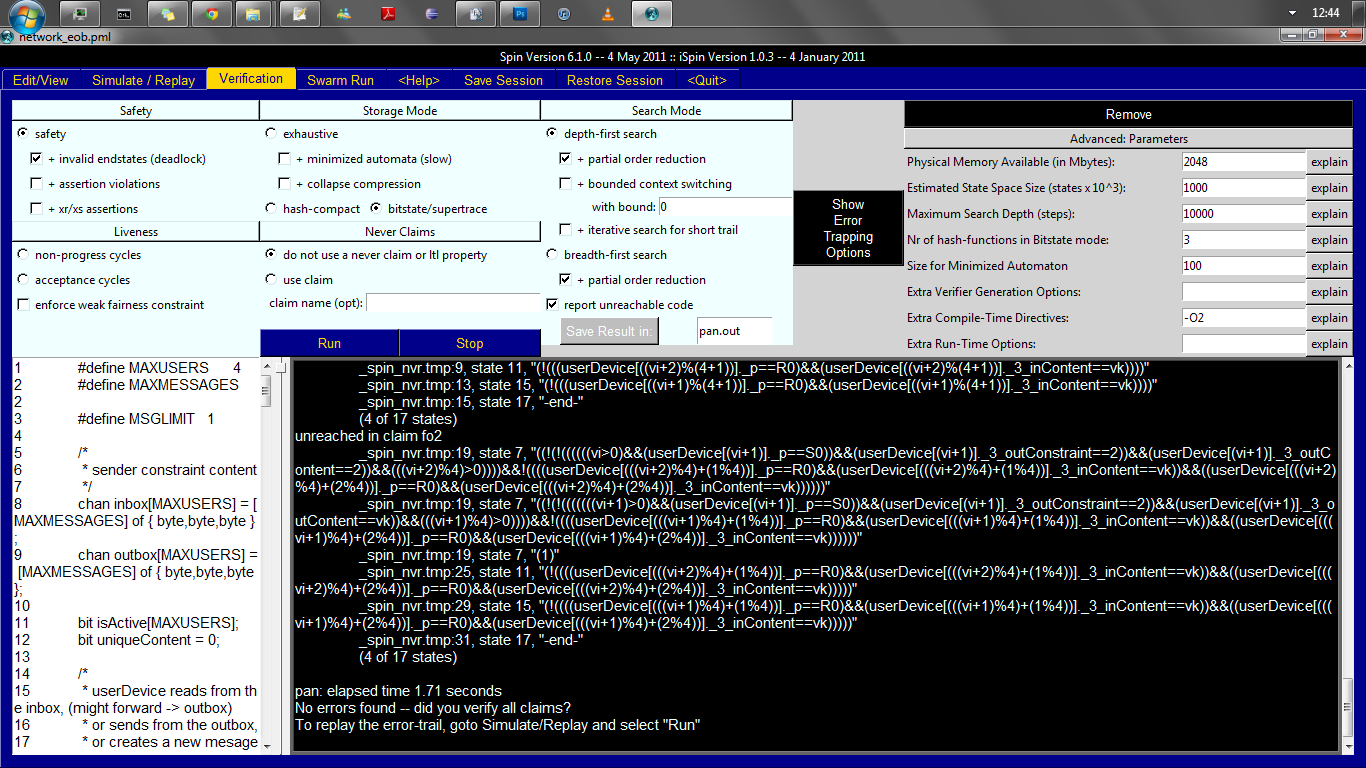
\includegraphics[angle=90,totalheight=\textheight]{screenshots/verification_safety.png}
		\caption{Verification for safety, checking deadlocks}
		\label{veriSafety}
	\end{figure}

	\begin{figure}[t]
		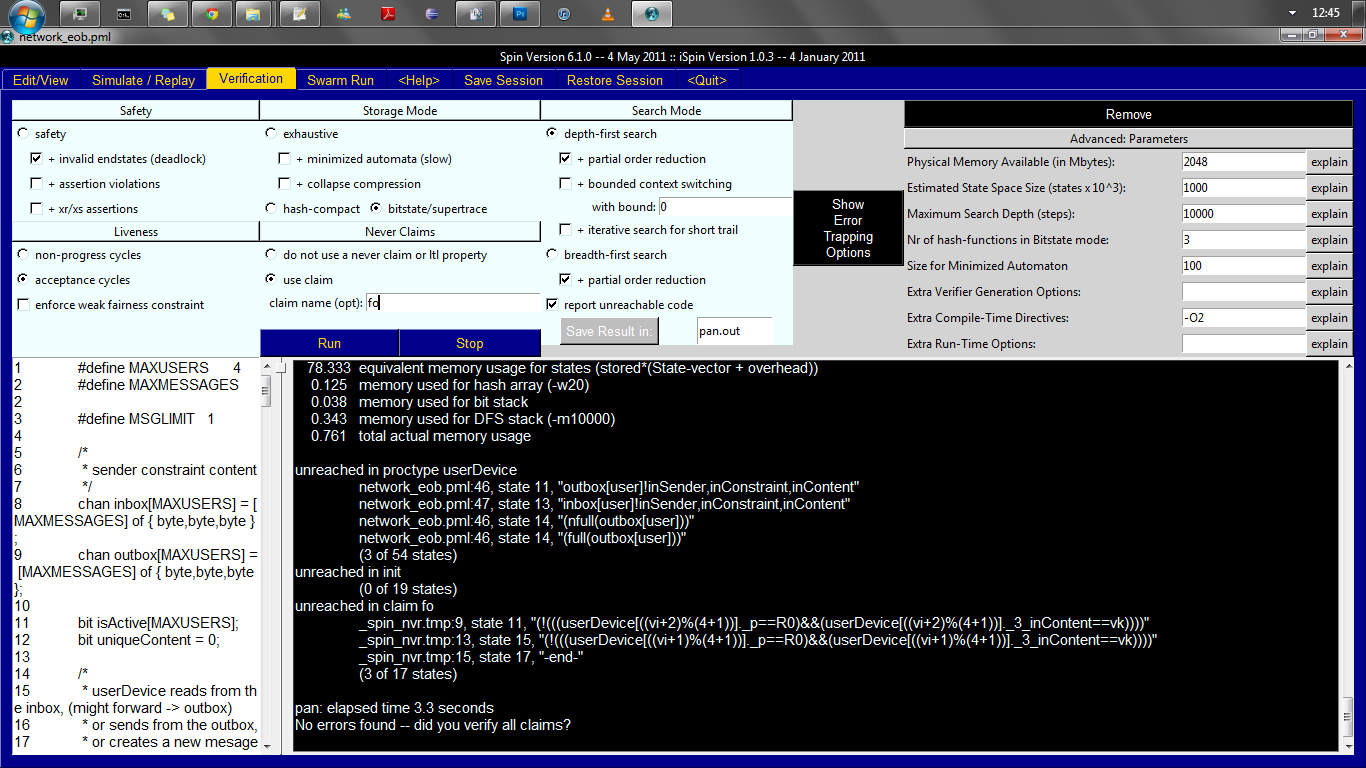
\includegraphics[angle=90,totalheight=\textheight]{screenshots/verification_fo.png}
		\caption{Verification for the Fo claim}
		\label{veriFo}
	\end{figure}
	
	\begin{figure}[t]
		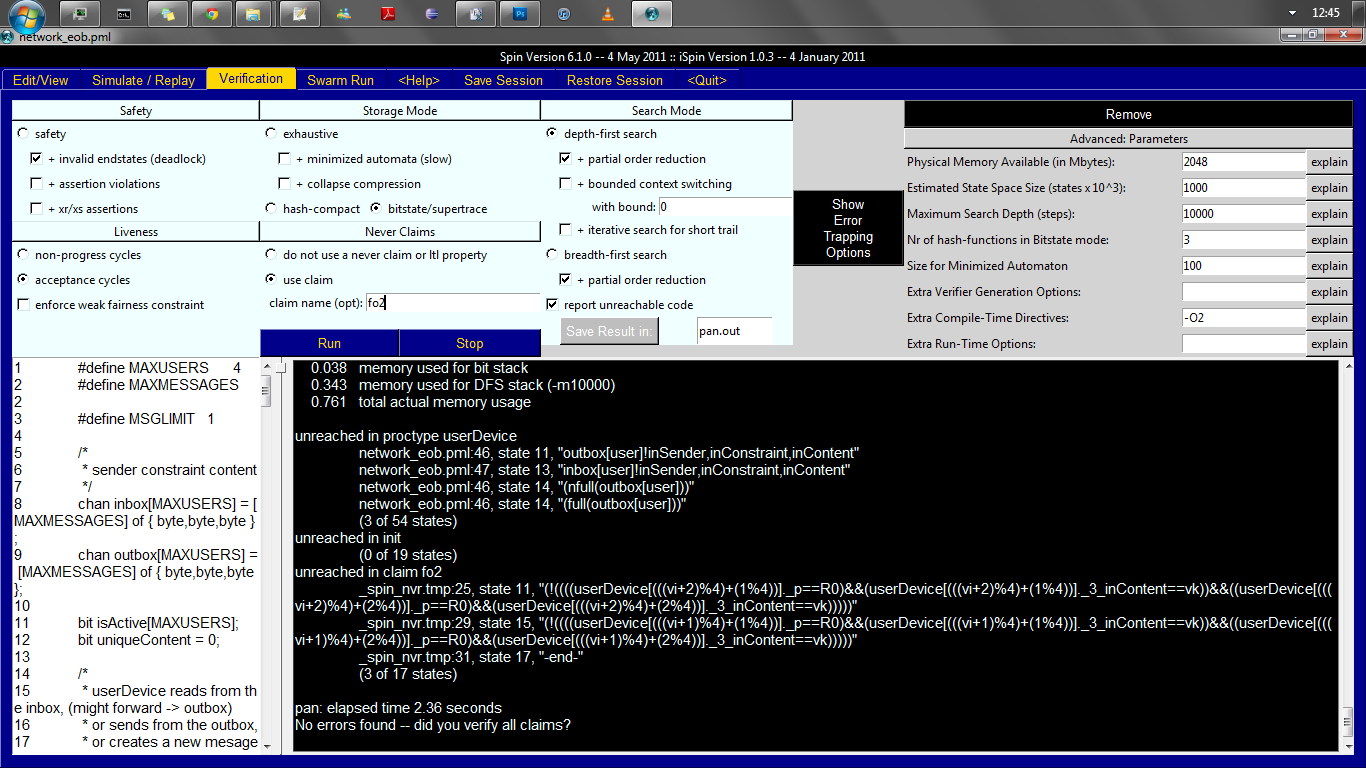
\includegraphics[angle=90,totalheight=\textheight]{screenshots/verification_fo2.png}
		\caption{Verification for the Fo2 claim}
		\label{veriFo2}
	\end{figure}
	
	\section{Code}
\lstinputlisting[language=Promela, breaklines=true,keywordstyle=\color{blue},commentstyle=\color{dkgreen}, stringstyle=\color{mauve}]{../network_final.pml}

	
\end{document}